\section{Results}
\label{hptpcPaper:sec:Results}

	\begin{figure}[ht]
		\begin{minipage}[t]{0.48\textwidth}
			\centering
			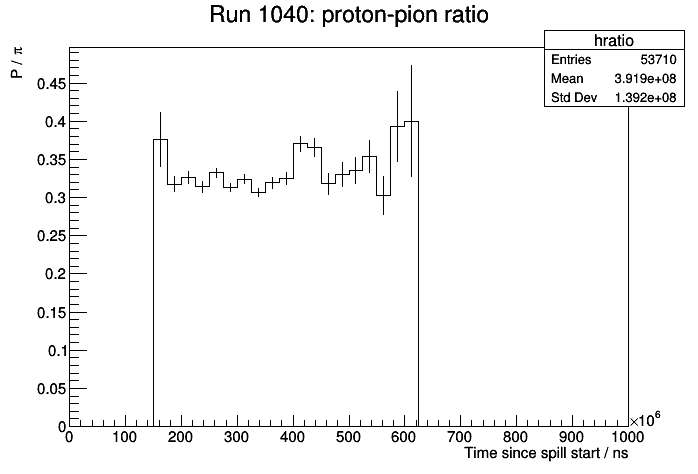
\includegraphics[width=\textwidth]{files/Figures/Run1040_proPiRatio}
			\caption{The ratio of protons to pions as a function of time since the start of the beam spill. For these data, 1 moderator block was in place and the beam momentum was nominally 0.8~GeV/c. The data for this graph is from the sum of 255 spills.}
			\label{fig:proPiRatio}
		\end{minipage} 
		\hspace{0.3cm}
		\begin{minipage}[t]{0.48\textwidth}
			\centering
			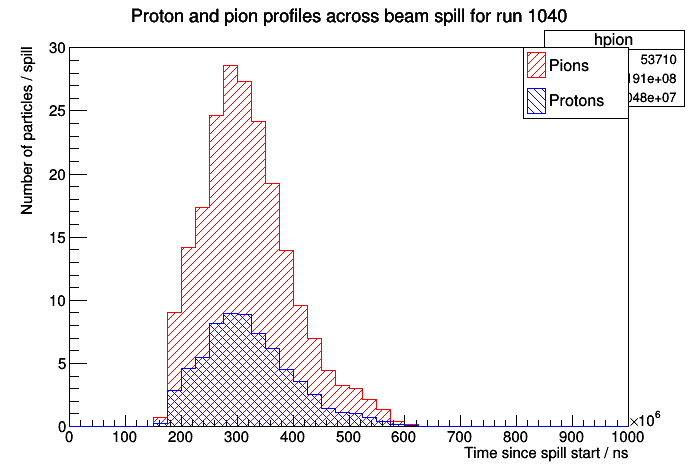
\includegraphics[width=\textwidth]{files/Figures/Run1040_proPiProf}
			\caption{The number of protons and pions detected per spill by the DsToF as a function of time since the start of the beam spill. For these data, 1 moderator block was in place and the beam momentum was nominally 0.8~GeV/c. The data for this graph is from the sum of 255 spills.}
			\label{fig:proPiProf}
		\end{minipage}
	\end{figure}

	Figure~\ref{fig:dtof_nmodblocks} shows the variation in the time of flight spectrum as recorded by the DsToF with a changing number of moderator blocks. The configuration used for most of the run was with 4 moderator blocks. 
			
	

   	\begin{figure}[h]
        \centering
	    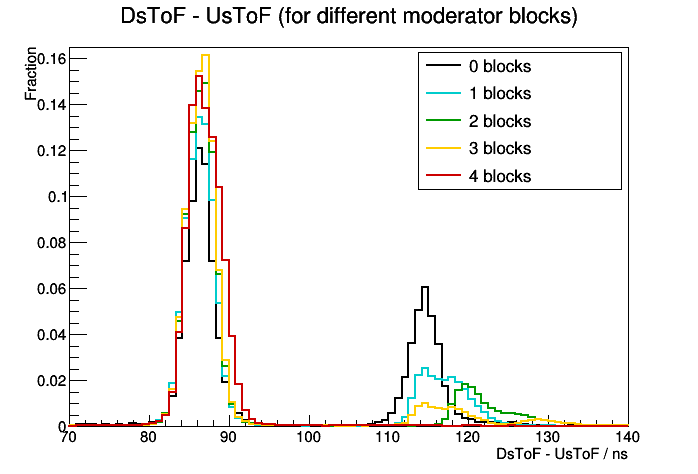
\includegraphics[width=0.7\linewidth]{files/Figures/AllInOne.png}
        \caption{Time of flight spectra for varying numbers of moderator blocks. For all configurations, the exposure has been normalised to one.}
        \label{fig:dtof_nmodblocks}	
   	\end{figure}
        
   	\begin{figure}[ht]
   		\begin{minipage}[t]{0.48\textwidth}
   			\centering
   			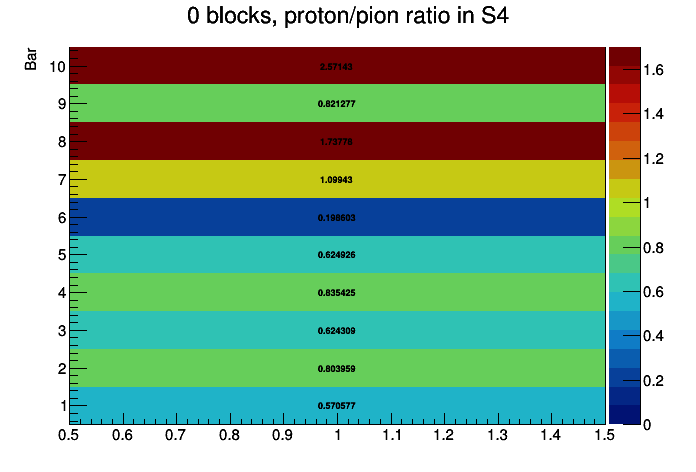
\includegraphics[width=\textwidth]{files/Figures/0blocks_propiratio_vert}
   			\caption{Proton:pion ratio with 0 moderator blocks}
   			\label{fig:0blocks_propiratio_vert}
   		\end{minipage}
   		\hspace{0.3cm}
    	\begin{minipage}[t]{0.48\textwidth}
    		\centering
    		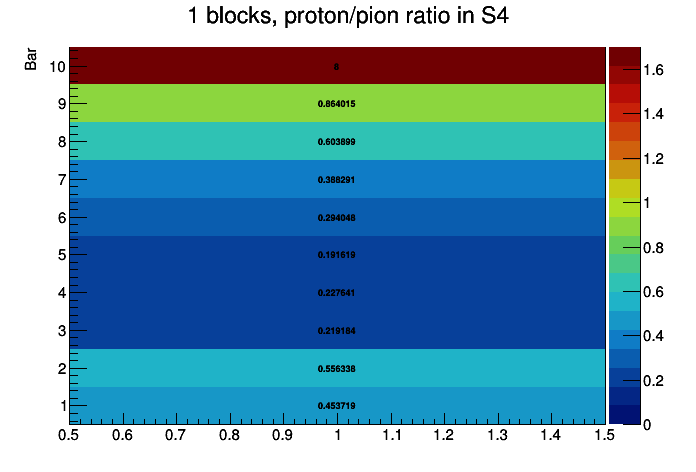
\includegraphics[width=\textwidth]{files/Figures/1blocks_propiratio_vert}
    		\caption{Proton:pion ratio with 1 moderator block}
    		\label{fig:1blocks_propiratio_vert}
    	\end{minipage}	\\
    	\begin{minipage}[t]{0.48\textwidth}
    		\centering
    		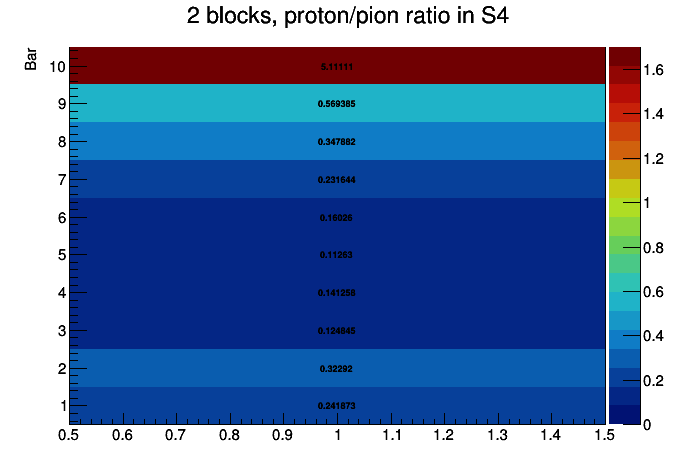
\includegraphics[width=\textwidth]{files/Figures/2blocks_propiratio_vert}
    		\caption{Proton:pion ratio with 2 moderator blocks}
    		\label{fig:2blocks_propiratio_vert}
    	\end{minipage}
    	\hspace{0.3cm}
    	\begin{minipage}[t]{0.48\textwidth}
    		\centering
    		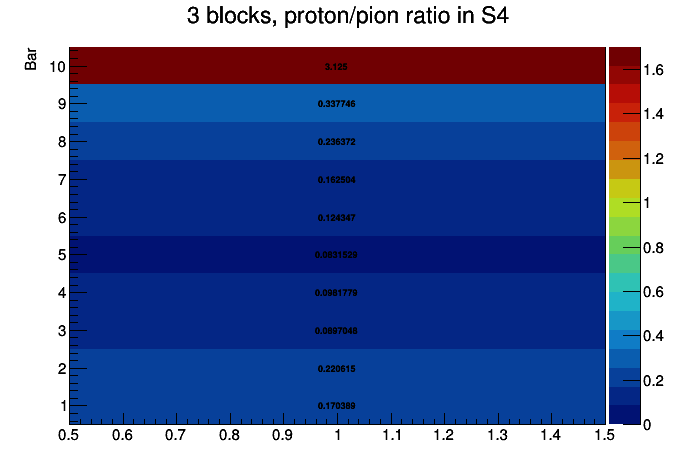
\includegraphics[width=\textwidth]{files/Figures/3blocks_propiratio_vert}
    		\caption{Proton:pion ratio with 4 moderator blocks}
    		\label{fig:4blocks_propiratio_vert}
    	\end{minipage}
   	\end{figure}
	

Exact UToF and DToF figures TBD